\chapter{BTF acquisition}
\label{chapter:acquisition}

BTF acquisition is not an easy task as it requires time for acquiring and post-processing the data, and also resources are needed to create acquisition setup.
There are only a few measurement systems \cite{star2004,schwartz,dana,Kaleidoscope,Koudelka,statistical_acq} exist, but as the interest in the realistic material rendering using BTF is growing, measurement systems are developing.
In this chapter we will review how in general BTF data acquisition is made, which post-processing steps are made, and pros and cons of existing measurement systems. 
Also, we will take a look at publicly available BTF datasets.

\section{General acquisition methods}
\label{section:General_acquisition}	
All the mentioned BTF acquisition systems share the same idea in the data acquisition, i.e. capturing the appearance of a flat square slice of the material surface under varying light and camera directions.
The material surface is usually sampled over a hemisphere above the material slice as shown in Figure \ref{fig:acquisition_example}.
Depending on the material reflectance properties sampling distribution may vary, e.g. sampling distribution can be dense in regions where specular peaks in light reflection occur. 
Then, if needed uniform distribution can be made in a post-processing step with a help of interpolation \cite{haindl_visual}.

Digital cameras are used as capturing devices of the material appearance. Depending on the setup the number of cameras can vary.
 If there is only one camera \cite{star2004,statistical_acq,dana}, it usually moves around over the hemisphere above the sample with a help of robotic arm or the rail-trail system \cite{star2004}. 
 The advantage of such approach is that it is less expensive and can suit for low-budget applications.
But, the disadvantage is the positioning errors that can arise, which influence the overall measurement error. 
Depending on the application light sources can be fixed or moveable.

There are approaches which do not involve camera and light source movement at all.
Schwartz et al. \cite{schwartz} developed a novel measurement system which uses a dense array of 151 camera, which are uniformly placed on hemispherical structure.
Flashes of the cameras are used as light sources. Such setup provide high angular and spatial resolutions.

Also, Ngan et al. \cite{statistical_acq} made a setup which does not involve camera movement by placing the planar slices of the material in a form of the pyramid.
Thus, such setup captures the material appearance for 13 different camera views at once. Light directions are sampled by hand-moved electronic flash.
The disadvantage of such setup is that it provides sparse angular resolutions, but depending on the application such approach can be plausible.

The material sample is commonly flat and squared slice, which is placed the holder plate. To conduct automatic post-processing borderline markers are placed on the holder.
Those markers provide the important information for further post-processing steps such as image rectification and registration.


\begin{figure}[h]
 \centering
 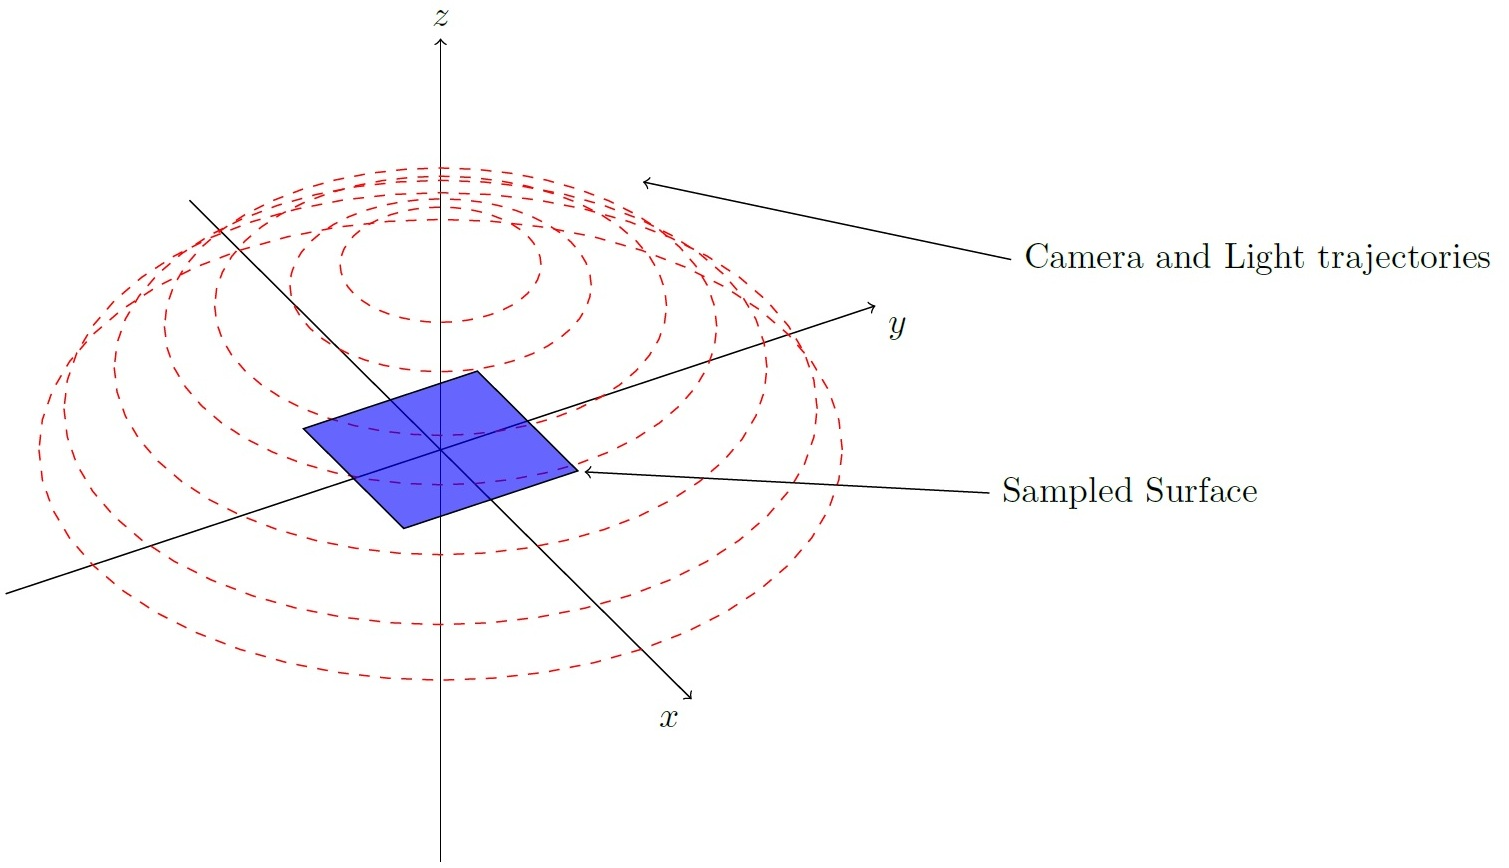
\includegraphics[width=1.0\textwidth]{figures/acquisition}
 \caption[Example of BTF measurement] {
 	{\bf Example of BTF measurement.}

	Camera and light positions share the same trajectories.
	Red dashed circles are the sample positions on the hemisphere. }
 \label{fig:acquisition_example}
\end{figure}

\section{Post-processing steps}
\label{section:Post_processing_acquisition}	
After the measurement is done, the raw data has to be further post-processed, because typically such such data is not ready for further modeling/compression or rendering.
Raw data is a set of images that are not aligned with each other and images are not mutually registered.

When the raw images are obtained under different camera angles $(\theta,\phi)$ they are perspectively distorted \cite{sattler-2003-efficient}.
Thus, sample image have to be aligned with each other and spatially registered to be further exploited.
Firstly, borderline markers that were placed around the material sample on the holder plate aid the automatic detection of the material slice.
Then, after the material slices are detected and cropped, they are ready to for mutual alignment. This process is called  \emph{rectification}. 
\emph{Rectification} is a process which involves projecting all sample images onto the plane which is defined by the frontal view, e.g. $(\theta _{o} =0,\phi _{o}=0)$.
In other words, all normals of sample images have to be aligned with their corresponding camera directions, i.e. as if all sample images were taken from frontal view $(\theta =0,\phi=0)$.
The last step is image \emph{registration}, a process of getting pixel-to-pixel correspondence between the images.
 As, all transformation were done, it is only enough to rescale all images to some equal resolution.


Even after the proper rectification and registering of the measured data, registration errors can be still present between individual camera directions \cite{haindl_visual}. 
 This happens due to structural occlusions of the material surface. Because, of such self-occlusions some geometry structures are not captured by certain camera directions, 
 but can be captured with other camera directions.
 That is why even after rectification images captured from completely different directions are not correctly mutually align. 
Also, registration errors can be caused both by inaccurate camera and material sample positions happened during the measurement processes.
One way to avoid artifacts in rendering caused by registration errors is to employ a compression step separately for each fixed camera positions, i.e. subsets of BTF data. 
 For instance, Sattler et. al. \cite{sattler-2003-efficient} has done this approach.


If needed, further processing steps can be done, for instance \emph{linear edger blending} to reduce tiling artifacts \cite{sattler-2003-efficient}.
Also, typical image processing steps may be employed, e.g. noise reduction filters. 


\section{Publicly available BTF datasets}
\label{section:Publicly_datasets}	

\begin{figure}[h]
 \centering
 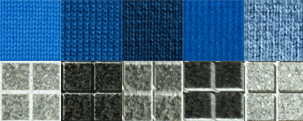
\includegraphics[width=1.0\textwidth]{figures/exampleBTF}
 \caption[Example of BTF measurement] {
 	{\bf BTF example of Bonn Database \cite{btfBonn}.}

	Example how BTF catches rich appearance of the material due to dependencies on light and camera directions. 
	Upper row is a knitted wool, lower is a graved granite stone.}
 \label{fig:exampleBTF}
\end{figure}


The accurate rendering of the material surface is highly depended on the quality of acquired data, especially for BTF.
There are several properties that are vital for reproducing quality rendering results.
The BTF datasets can be distinguished by how well image post-processing were done and how good spatial and angular resolutions are.
So, depending on the application trade-off between high and low spatial or angular resolutions is done.
 For example, some materials with a low range of reflectance may benefit from sparse resolutions, e.g. wool, plastic, etc.
 
 
A pioneer in the BTF acquisition was Dana et. al. \cite{curetDataBase}, who measured 61 materials with fixed light and moving camera aided by a robotic arm. 
Such procedure resulted in a set of images, which can be regarded as a subset of BTF, which is called reflectance field (RF)

{\centering $RF(x,y,\theta _{i},\phi _{i},\theta _{o},\phi _{o})$ \\}

where $(x,y)$ is a surface point of a flat sampled material, $(\theta _{i},\phi _{i})$ incoming light direction (light direction) and $(\theta _{o},\phi _{o})$ outgoing light direction (camera direction).

Data et. al. \emph{CUReT} database is publicly available \cite{curetDataBase}.
For each measured surface Dana et. al. used 205 different combinations of camera and light directions, which resulted in relatively sparse angular resolution.
 Dana's et. al. BTF database are not rectified, but  the authors provide image coordinates to allow their further rectification. 
 Because, of this limitations such BTF dataset usually used for computer vision purposes, i.e. texture classification  \cite{haindl_visual}.

Based on Dana et. al. BTF measurement system, Sattler from Bonn University made his own measuring system \cite{sattler-2003-efficient}.
 The main difference in that system is that a camera moves on a semi-circle rail around material sample.
Such setup provides spatially rectificated and mutually registered data, with reasonable angular and spatial resolutions. 
Datasets of Bonn University \cite{btfBonn} are publicly available and were used in this thesis.


 Consider Figure \ref{fig:exampleBTF}, which illustrates one of the sampled materials of Bonn database.
The measured surface is being fixed all the time on the sampler holder as shown in Figure \ref{fig:acquisition_example}. For each light position, a camera takes a shot of the material while moving from point to point of the hemisphere.
Bonn database has the same trajectory for camera and light positions, i.e. 81 positions on the hemisphere, which resulted in $81\times81=6561$ total number of acquired images.
After that the sample images were rectificated and registered, resulting in a set of images with spatial resolution $256\times256$.
Typically, the size of one uncompressed BTF is around $1.2$ Gb.






